%%
%% This is file `sample-manuscript.tex',
%% generated with the docstrip utility.
%%
%% The original source files were:
%%
%% samples.dtx  (with options: `manuscript')
%% 
%% IMPORTANT NOTICE:
%% 
%% For the copyright see the source file.
%% 
%% Any modified versions of this file must be renamed
%% with new filenames distinct from sample-manuscript.tex.
%% 
%% For distribution of the original source see the terms
%% for copying and modification in the file samples.dtx.
%% 
%% This generated file may be distributed as long as the
%% original source files, as listed above, are part of the
%% same distribution. (The sources need not necessarily be
%% in the same archive or directory.)
%%
%% Commands for TeXCount
%TC:macro \cite [option:text,text]
%TC:macro \citep [option:text,text]
%TC:macro \citet [option:text,text]
%TC:envir table 0 1
%TC:envir table* 0 1
%TC:envir tabular [ignore] word
%TC:envir displaymath 0 word
%TC:envir math 0 word
%TC:envir comment 0 0
%%
%%
%% The first command in your LaTeX source must be the \documentclass command.
%%%% Small single column format, used for CIE, CSUR, DTRAP, JACM, JDIQ, JEA, JERIC, JETC, PACMCGIT, TAAS, TACCESS, TACO, TALG, TALLIP (formerly TALIP), TCPS, TDSCI, TEAC, TECS, TELO, THRI, TIIS, TIOT, TISSEC, TIST, TKDD, TMIS, TOCE, TOCHI, TOCL, TOCS, TOCT, TODAES, TODS, TOIS, TOIT, TOMACS, TOMM (formerly TOMCCAP), TOMPECS, TOMS, TOPC, TOPLAS, TOPS, TOS, TOSEM, TOSN, TQC, TRETS, TSAS, TSC, TSLP, TWEB.
% \documentclass[acmsmall]{acmart}

%%%% Large single column format, used for IMWUT, JOCCH, PACMPL, POMACS, TAP, PACMHCI
% \documentclass[acmlarge,screen]{acmart}

%%%% Large double column format, used for TOG
% \documentclass[acmtog, authorversion]{acmart}

%%%% Generic manuscript mode, required for submission
%%%% and peer review

\documentclass[manuscript,screen,review]{acmart} % twocolumn
\usepackage{graphicx}
\usepackage{subcaption}
\usepackage{todonotes}
\usepackage{hyperref}
\usepackage{etoolbox}
\usepackage{multicol}


% \preto{\section}{\clearpageafterfirst}
% \preto{\subsection}{\filbreak}
% \newcommand{\clearpageafterfirst}{%
%   \gdef\clearpageafterfirst{\clearpage}%
% }

%% Fonts used in the template cannot be substituted; margin 
%% adjustments are not allowed.
%%
%% \BibTeX command to typeset BibTeX logo in the docs
\AtBeginDocument{%
  \providecommand\BibTeX{{%
    \normalfont B\kern-0.5em{\scshape i\kern-0.25em b}\kern-0.8em\TeX}}}

%% Rights management information.  This information is sent to you
%% when you complete the rights form.  These commands have SAMPLE
%% values in them; it is your responsibility as an author to replace
%% the commands and values with those provided to you when you
%% complete the rights form.
\setcopyright{acmlicensed}
\copyrightyear{2018}
\acmYear{2018}
\acmDOI{XXXXXXX.XXXXXXX}

%% These commands are for a PROCEEDINGS abstract or paper.
\acmConference[Conference acronym 'XX]{Make sure to enter the correct
  conference title from your rights confirmation emai}{June 03--05,
  2018}{Woodstock, NY}
%
%  Uncomment \acmBooktitle if th title of the proceedings is different
%  from ``Proceedings of ...''!
%
\acmBooktitle{Woodstock '18: ACM Symposium on Neural Gaze Detection,
 June 03--05, 2018, Woodstock, NY} 
\acmISBN{978-1-4503-XXXX-X/18/06}

%%
%% Submission ID.
%% Use this when submitting an article to a sponsored event. You'll
%% receive a unique submission ID from the organizers
%% of the event, and this ID should be used as the parameter to this command.
%%\acmSubmissionID{123-A56-BU3}

%%
%% For managing citations, it is recommended to use bibliography
%% files in BibTeX format.
%%
%% You can then either use BibTeX with the ACM-Reference-Format style,
%% or BibLaTeX with the acmnumeric or acmauthoryear sytles, that include
%% support for advanced citation of software artefact from the
%% biblatex-software package, also separately available on CTAN.
%%
%% Look at the sample-*-biblatex.tex files for templates showcasing
%% the biblatex styles.
%%

%%
%% The majority of ACM publications use numbered citations and
%% references.  The command \citestyle{authoryear} switches to the
%% "author year" style.
%%
%% If you are preparing content for an event
%% sponsored by ACM SIGGRAPH, you must use the "author year" style of
%% citations and references.
%% Uncommenting
%% the next command will enable that style.
%%\citestyle{acmauthoryear}

%%
%% end of the preamble, start of the body of the document source.
\begin{document}

% \begin{multicols}{2}

%%
%% The "title" command has an optional parameter,
%% allowing the author to define a "short title" to be used in page headers.
\title[Trainieren Neuronaler Netze zur Klimavorhersage}

%%
%% The "author" command and its associated commands are used to define
%% the authors and their affiliations.
%% Of note is the shared affiliation of the first two authors, and the
%% "authornote" and "authornotemark" commands
%% used to denote shared contribution to the research.
\author{Torge Schwark}
\authornote{Both authors contributed equally to this research.}
\email{stuTODO:@mail.uni-kiel.de}
\orcid{1234-5678-9012}
\author{Joschua Quotschalla}
\authornotemark[1]
\email{stu235352@mail.uni-kiel.de}
\affiliation{%
  \institution{Institute of Computer Science, University of Kiel}
  \streetaddress{P.O. Box 1212}
  \city{Kiel}
  \state{Schleswig-Holstein}
  \country{Germany}
  \postcode{2411TODO:}
}

% %% TODO: Text in grau markiert unsichere/zu überarbeitende Stellen
% \begin{abstract}
% In Anbetracht der globalen Bedeutung und Auswirkungen des Klimawandels sind präzise Vorhersagen der zukünftigen Klimaentwicklung von entscheidender Bedeutung. 
% Die vorliegende Studie konzentriert sich auf die Anwendung von neuronalen Netzwerken zur Klimavorhersage, 
% wobei der umfangreiche Datensatz "Climate Change: Earth Surface Temperature Data" als Grundlage dient. 
% Durch die systematische Verwendung verschiedener Architekturen, darunter Multilayer-Perzeptronen (MLPs), Long Short-Term Memory Networks (LSTMs), 
% Convolutional Neural Networks (ConvNets) und Transformer-Modelle, wird das Ziel verfolgt, 
% präzise und langfristige Vorhersagen zur \textcolor{gray}{globalen Durchschnittstemperatur für die kommenden 100 Jahre zu ermöglichen.}
% \textcolor{gray}{Mit Blick auf die Dringlichkeit des Themas Klimawandel soll dieses Paper einen differenzierten Einblick in die Anwendung neuronaler Netze für die Klimavorhersage bieten. 
% Der Fokus liegt dabei nicht nur auf der Vorhersage zukünftiger Temperaturentwicklungen, sondern auch auf der Identifizierung langfristiger globaler Trends.} 
% Die Bedeutung und weitreichenden Folgen des Klimawandels für Mensch und Umwelt unterstreichen die Notwendigkeit, präzise und zuverlässige Vorhersagemodelle zu entwickeln, 
% um fundierte Entscheidungen und Maßnahmen treffen zu können.
% Neben der Motivation zur Untersuchung des Klimawandels aus datengetriebener Sicht werden in diesem Paper auch Einblicke in die angewandten Methoden, 
% den verwendeten Datensatz, den Trainingsprozess, die erzielten Ergebnisse und abschließende Schlussfolgerungen präsentiert. Das übergeordnete Ziel besteht darin, 
% einen bedeutenden Beitrag zur Vorhersage zukünftiger Klimaentwicklungen zu leisten und damit einen wertvollen Beitrag zum besseren Verständnis und zur Bewältigung des Klimawandels zu leisten.
% \textcolor{gray}{Diese Studie erstreckt sich über insgesamt 6 getippte Seiten, wobei dieser einleitende Abschnitt den notwendigen Rahmen für das folgende Forschungspapier bildet.}
% \end{abstract}

\keywords{neuronale Netzwerke, NN, MLP, 1D CONV, LSTM, Transformer, Klimawandel, Temperatur}

%% A "teaser" image appears between the author and affiliation
%% information and the body of the document, and typically spans the
%% page.
% \begin{teaserfigure}
%   
\includegraphics[scale=0.1]{./sources/NN_climate_icon.jpg}
%   \caption{Seattle Mariners at Spring Training, 2010.}
%   \Description{Enjoying the baseball game from the third-base
%   seats. Ichiro Suzuki preparing to bat.}
%   \label{fig:teaser}
% \end{teaserfigure}

% \received{20 February 2007}
% \received[revised]{12 March 2009}
% \received[accepted]{5 June 2009}

%%
%% This command processes the author and affiliation and title
%% information and builds the first part of the formatted document.
\maketitle

\todo{Wohin damit??}
\section{Glossar}
... Abkürzungen hier

% \section{Einleitung



\section{Einleitung}
Der Klimawandel stellt zweifellos eine der größten Herausforderungen des 21. Jahrhunderts dar. Der rapide Anstieg globaler Durchschnittstemperaturen und die daraus resultierenden Auswirkungen auf Umwelt und Gesellschaft erfordern dringendes Handeln. Als Grundlage für präventive Maßnahmen ist ein umfassendes Verständniss und das erkennen langfristiger Klimatrends zwingend notwendig. 
Die Anwendung neuronaler Netze verspricht nicht nur verbesserte Vorhersagegenauigkeit, sondern eröffnet auch die Möglichkeit, bisher unbekannte Muster und Trends zu identifizieren, die für ein umfassenderes Verständnis des Klimawandels von entscheidender Bedeutung sind.

\subsection{Schwerpunkt: Das Training Neuronaler Netze}
Der Fokus dieser Untersuchung liegt auf dem Training neuronaler Netze, um eine möglichst hohe Vorhersagegenauigkeit zu erzielen. Dabei werden die Architekturtypen MLP, ConvNet, LSTM und Transformer darauf trainiert, eine Klimavorhersage über 25 Jahre zu treffen. Anschließend werden die Ergebnisse analysiert und die Performance der trainierten neuronalen Netze miteinander verglichen. 

\subsection{Ziel}
Das Ziel besteht darin, mithilfe des besten neuronalen Netzes eine aussagekräftige Vorhersage für die Klimaentwicklung der nächsten 100 Jahre zu treffen.
Die folgenden Abschnitte werden detailliert auf die verwendeten Methoden, die Datenaufbereitung, den Trainingsprozess, die Ergebnisse und die abschließende Schlussfolgerung eingehen.
]


\section{Methoden}

\subsection*{Datensatz und Datenaufbereitung}
\begin{itemize}
    \item Umfassende Analyse des Datensatzes: Histogramme, Barcharts, Landkarten.
    \item Überprüfung auf Duplikate, insbesondere gleiche Städte.
    \item Aufteilung in Trainings- und Validierungssets (70/30).
    \item Filterung von Zeiträumen mit konstanten Daten über 95 Jahre.
\end{itemize}

\subsection*{Training der neuronalen Netze}
\begin{itemize}
    \item Berechnung des MAE über 720 menschliche Vorhersagen als Bezugsgröße.
    \item Anwendung einer Grid Search-Methode für MLPs, ConvNets, LSTMs.
    \item Feintuning: Anpassung von Hyperparametern, Augmentation, Normalisierung.
\end{itemize}

\subsection*{Auswertung}
\begin{itemize}
    \item Prüfen auf Overfitting, Analyse des Loss Graphen.
    \item Vergleich des MAE mit menschlichen Vorhersagen.
    \item Analyse der Genauigkeit an Beispielen.
\end{itemize}

\subsection*{Anwendung}
\begin{itemize}
    \item Anwendung des besten Netzwerks für Vorhersagen bis 2110.
    \item Erstellung eines Durchschnittsgraphen von 1750 bis 2110 mittels rolling prediction.
\end{itemize}

\section{Datensatz}
\subsection{Einführung und Datenverständnis}
Die Grundlage dieser Studie bildet der \href{https://www.kaggle.com/datasets/berkeleyearth/climate-change-earth-surface-temperature-data?select=GlobalLandTemperaturesByCity.csv}{"Climate Change: Earth Surface Temperature"} Datensatz.
Der genannte Datensatz umfasst insgesamt 10.064.718 monatliche Durchschnittstemperaturen, die in 3.448 Städten von 159 Ländern erhoben wurden. Die Aufzeichnungen reichen dabei von den frühesten Daten im Jahr 1743 bis zu den aktuellsten im Jahr 2015.

\subsection{Fehlende Daten und Ungenauigkeiten}
Bei unserer Analyse auf Duplikate stellten wir fest, dass 117 Städte im Datensatz doppelt oder mehrfach vorkommen. Dabei wurden Duplikate erkannt, falls die Daten zweier Städte vollständig identisch sind.  Diese doppelten Einträge sind vermutlich auf die Tatsache zurückzuführen, dass der Datensatz eine Zusammenstellung von 16 bereits bestehenden Datenarchiven darstellt. Im Datensatz sind zu den jeweiligen durchschnittlichen Temperaturen auch die durchschnittlichen Messunsicherheiten aufgeführt. Obwohl diese Unsicherheiten stetig abnehmen, stellen sie dennoch eine Herausforderung für die Vorhersagegenauigkeit dar. dabei ist zu beachten, dass der exakte Messwert mit hoher Wahrscheinlichkeit eine geringere Abweichung aufweist als die Messunsicherheit. Daher ist der durchschnittliche Messfehler deutlich geringer als die Messunsicherheit.
Das bedeutet, das der Zufallsfaktor, der durch ungenaue Messungen entsteht und eine untere Schranke für die Vorhersagegenauigkeit bildet nicht der angegebenen Messunsicherheit endspricht.

\subsection{Data-Loader Pipeline} % noch überarbeiten
Die Data-Loader Pipeline wurde implementiert, um Mini-Batches von Sequenzen von Datenpunkten gemäß den Anforderungen der Architekturen bereitzustellen. Dabei muss sichergestellt werden, dass Datenpunkte für die gesammte input länge von 70 Jahren(840 Monaten) und output länge von 25 Jahren(320 Monate) ohne Lücken vorhanden sind.
Um die Effizienz des Trainings zu steigern, erfolgte die Extraktion der Daten aus den fünf CSV-Dateien, wobei für jeden Standort eine eigene Textdatei angelegt wurde. Zu Beginn wählten wir einen zufälligen Standort und einen zufälligen Zeitraum in dem 90 Jahre vollstänige Messwerte vohanden waren.
Später versuchten wir den Data-Loader weiter zu verbessern, dazu speicherten wir die gesamten Daten zunächst in Listen und führten die Suche nach passenden Zeiträumen einmalig am Anfang des Trainings durch. Diese Optimierung brachte jedoch nicht den gewünschten Effekt.

Die spätere Anwendung von Multiprocessing zur Ausführung des Data-Loaders auf bis zu 20 Prozessen gleichzeitig, beschleunigte den Data-Loader mit minimalem Aufwand um etwa das Zehnfache und erhöhte die Hardware-Auslastung merklich. Der Flaschenhals lag dabei im Arbeitsspeicher.


\section{Visualisierungen für Datenanalyse und Predictions}

\todo{richtigen Histogramme hinzufügen}
\begin{figure}[htp]
  \centering
  \begin{subfigure}{.45\textwidth}
      \centering
      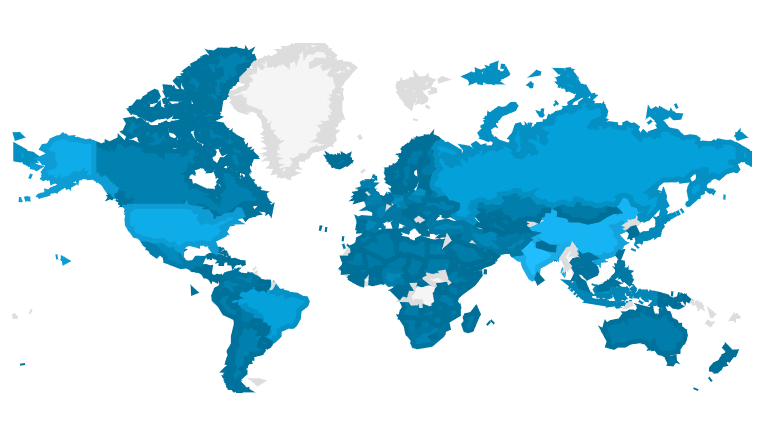
\includegraphics[width=.8\linewidth]{./map_plot_data_points}
      \caption{Ursprung Daten}
      \label{fig:sub1}
  \end{subfigure}%
  \begin{subfigure}{.45\textwidth}
      \centering
      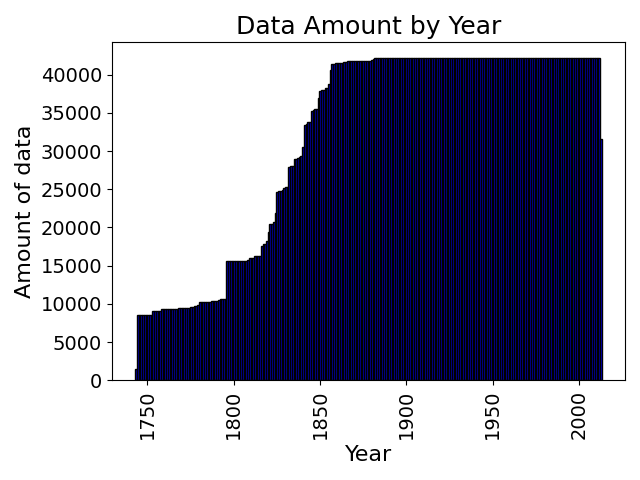
\includegraphics[width=.8\linewidth]{./Years}
      \caption{Anzahl Daten}
      \label{fig:sub2}
  \end{subfigure}\\
  \begin{subfigure}{.45\textwidth}
      \centering
      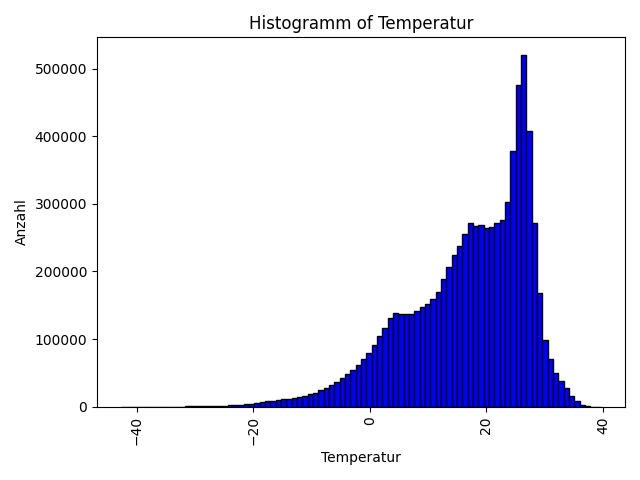
\includegraphics[width=.8\linewidth]{./Temperatur}
      \caption{Histogram 3}
      \label{fig:sub3}
  \end{subfigure}%
  \begin{subfigure}{.45\textwidth}
      \centering
      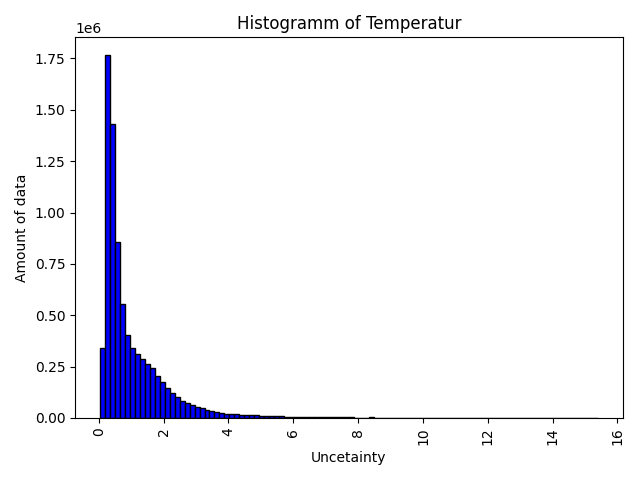
\includegraphics[width=.8\linewidth]{./Uncertainty}
      \caption{Unsicherheiten}
      \label{fig:sub4}
  \end{subfigure}
  \caption{Four histograms}
  \label{fig:test}
  \Description{Histograms caputuring the distribution of the data.}
\end{figure}

\subsection{Histogramm Ursprung Daten}
\todo{Beschreibung / Deutung}

\subsection{Histogramm Anzahl Daten}
\todo{Beschreibung / Deutung}

\subsection{Histogramm Uncertainty}
\todo{Beschreibung / Deutung}

\subsection{Histogramm Datagaps}
\todo{Beschreibung / Deutung}


\section{Training-Procedure}

Um Klimaprognosen zu erstellen wurden die Architekturtypen MLP, ConvNet, LSTM und Transformer trainiert, auf einem Input von 70 Jahren(840 Monaten) eine Vorhersage für die Nächsten 25 Jahre(300) Monate zu treffen.
Im ersten Schritt wurde eine Grid Search durchgeführt, um optimale Modelle und deren Hyperparameter für die jeweiligen Architekturtypen zu aproximieren. 
Nach dieser automatisierten Suche wurde ein händisches Fine-Tuning durchgeführt, um die Leistung der Modelle weiter zu verbessern. 
Während des gesamten Prozesses wurde darauf geachtet, wie sich jede Architektur an die spezifischen Charakteristiken des Datensatzes anpasst und 
wie gut sie die Temperaturvorhersagen durchführen kann.

\subsection{Optimierung von Architekturen und Parametern}
Die Auswahl und Optimierung der geeigneten Parameter für neuronale Netzwerkarchitekturen spielt eine entscheidende Rolle bei der Leistungsfähigkeit und Zuverlässigkeit der Klimavorhersagemodelle. 
Im Rahmen der Untersuchung wurden verschiedene \textcolor{gray}{Schlüsselparameter/Hyperparameter} betrachtet und optimiert, um die bestmöglichen Ergebnisse zu erzielen.
Dazu gehören zum einen allgemein Parameter wie etwa die Batchsize, Anzahl der Epochen, Steps pro Epoche, Anzahl der validierungs Steps und das Verhältniss von Trainingsdaten zu Validierungsdaten.
Weiterhin besitzen die genannten Architekturen auch eigene exklusive Charakteristiken, welche einen enormen Einfluss auf die Performance haben und dementsprechend im folgenden genauer untersucht werden.

\subsection{Allgemeine Parameter / Settings} \todo{Batchsize / Steps dynamisch anpassen}

Da im Training als erstes eine Grid Search durchgeführt wurde und in dieser ausschließlich die Auswirkung der verschiedener Architekturen, Batch sizes und Learning rates auf den MAE untersucht wurden, mussten die restlichen Parameter zunächst festgelegt werden. Dabei wurde sich auf die bereits erwähnte Input- und Output-Länge, die Aufteilung des Datensatzes in 70 Prozent zum Trainieren und 30 Prozent zum Validieren und die Patience von 10 Epochen geeinigt. Durch die Patience wird sichergestellt, dass das Training erst nach 10 Epochen ohne eine Verbesserung des MAEs beendet wird. Des Weiteren wurden damit die Geschwindigkeit des Trainings vergleichbar, auch wurden die Steps/Epoche dynamisch an die Batch size angepasst, sodass unabhängig von der Batch Size pro Epoche die gleiche Menge an Daten betrachtet werden. Wie jedoch später in der Auswertung zu sehen ist, ist auch dieses Vorgehen im Vergleich zu den verschiedenen Batch sizes nicht unbedingt fair. 

\todo{hier doch trotzdem als "Setting sinnvoll und nicht bei Results right?"} Weiterhin wurde eine adaptive Learningrate definiert, welche in Abhängigkeit von der Epoche entweder bei \textcolor{darkgray}{$epoche < 10$} den gegeben Learningrate Wert besitzt oder im \textcolor{darkgray}{$epoche \geq 10$} Fall \textcolor{darkgray}{learningrate = learningrate $\cdot e^{-0.1}$} setzt. Dies ermöglicht ein bei größeren Epochen präziseres Lernen.

\todo{Sollen die Architekturen mit den Hyperparametern in eine Tabelle??}

\subsection{Analyse von Architekturen}

\subsubsection*{MLP (Multilayer-Perzeptronen)}
Im Kontext von Multilayer-Perzeptronen (MLPs) spielen insbesondere die Anzahl der Hidden Layer in Kombination mit Dropout Layern und die Anzahl der Neuronen pro Layer eine bedeutsame Rolle bei der Optimierung.
\todo{soll das eher in die Results?}Allgemein lässt sich dabei beobachten, dass MLPs eine grundsätzlich gleichbleibende Stabilität der Performance innerhalb der Grid Search und explizit bei der Loss-Kurve des Trainings bieten, was darauf schließen lässt, dass diese Modelle eine relativ passende Kapazität im Bezug auf die Daten aufweisen. So sind viele der getesteten Modelle schon ab einer Epoche von 4-5 in einem sehr niedrigen Loss-Bereich. \todo{Loss-curve Grafik einbinden?} Im Zusammenhang damit ist auch die Dauer insbesondere mit einer Epochendauer von ~3 Sekunde bei den besser performenden Architekturen enorm gering.
Durch geziehltes Finetuning konnte somit der MAE von 1.1 auf 0.88 reduziert werden.
Dabei sieht die entstandene am besten performende Architektur mit Finetuning wie folgt aus:
\begin{itemize}
    \item Layer mit Anzahl an Neuronen: [500, 500, 500, 500, 500, 500, 500]
    \item Learning rate: 0.00008
    \item Augmentation: \todo{Wert}
    \item Earlystopping patience: 40
    \item Batch Size: 300
    \item Verbesserung durch gezieltes Finetuning (MAE): 0.86 $\rightarrow$ 0.83
\end{itemize}

\todo{Visualiierung der Architektur einbinden?}
\todo{Weiter Erläutern}
\todo{Flatten am Anfang}

\subsubsection*{1D-Convolutional Neural Networks (1D-ConvNets)}
Für 1D-ConvNets sind insbesondere die Größe und Anordnung der ilter sowie deren Anzahl in den Convolutional Layern und dem darauf folgendem MLP von großer Bedeutung. 
Während größere Filter und eine höhere Anzahl von Filtern zu einer komplexeren Modellarchitektur und möglicherweise zu einer besseren Erfassung räumlicher Merkmale führen können, haben sich trotzdem allgemein eher kleinere Filterrößen in den state of the art Modellen bewährt, welche wiederum ein detailierteres Verständnis für den input liefern können.
Somit wurden zunächst Modelle mit Kernels der Größe 3 und 5 getestet, welche aber im Vergleich zu den danach getesteten Architekturen mit Kernelgrößen bis zu 10 deutlich schlechter abschnitten. Das ist mit der schon erwähnten besseren Erfassung von räumlichen Merkmalen zu begründen, da ein Datenpunkte immer der Durchschnittswert eines Monats ist und Vorhersagen über viele Jahre nicht mehr den Verlauf von Temperaturen über wenige Monate sondern z.B. eines ganzen Jahres vorraussetzen.
Ein weiterer noch viel größerer Faktor bei den 1D-ConvNets Architekturen war der Layer zwischen den Convolution Layers und dem \textcolor{gray}{Dense/}MLP-Teil, welcher zum Beispiel ein 1D global average pooling oder ein Flatten sein konnte. Dabei schnitt das 1D global average pooling deutlich schlechter ab, sodass viele Modelle einen MAE von ~30 hatten und der beste erreichte MAE ~4.5 war, wohingegen durch ein Flatten Layer MAEs von unter 1 erreicht werden konnten. Dies lässt darauf schließen, dass ein 1D global average pooling einen signifikanten Anteil an Informationen verloren gehen lässt. Wieder im Vergleich dazu bietet Flatten durch ein simples aneinanderreihen von Zeilen der letzten Featuremaps den vollen Informationsumfang, sodass der folgende \textcolor{gray}{Dense/}MLP-Teil mit den extrahierten Features besser weiterarbeiten kann.
\todo{soll das eher in die Results?} Analog zu den MLPs waren auch die 1D-ConvsNets nach dem Umstieg auf Flatten sehr konsistent stabil im Training und wiesen mit einer Epochendauer von ~3 Sekunden ein schnelles Training auf. \todo{es gab modelle mit bestimmten punkt, wo performance signifikant besser wurde (auch siehe LSTM)}
Die am besten abschneidende Architektur mit Finetuning sieht wie folgt aus:
\begin{itemize}
    \item Anzahl Kernels pro Layer: [10, 10, 10, 10]
    \item Kernelgrößen pro Layer: [5, 5, 5, 5]
    \item MLP Anzahl Neuronen: \todo{bekannt?}
    \item Learning rate: 0.00005
    \item Augmentation: \todo{Wert}
    \item Earlystopping patience: 40
    \item Batch Size: 300
    \item Verbesserung durch gezieltes Finetuning (MAE): 0.86 $\rightarrow$ 0.8365
\end{itemize}

\todo{Visualiierung der Architektur einbinden?}
\todo{Weiter Erläutern}

\subsubsection*{LSTMs (Long Short-Term Memory Networks)}
Bei den LSTMs hingegen ist ein zentraler Parameter die Anzahl der Memory Units. Durch gezielte Anpassung dieser Anzahl kann die Netzwerkleistung verbessert und die Fähigkeit zur Erfassung von langfristigen Abhängigkeiten gesteuert werden. Nach den LSTM Layern folgt wieder ein \textcolor{gray}{Dene/}MLP-Teil. \todo{warum auch hier wieder MLP-Teil?}
In dem Experimenten wurde festgestellt, dass ... .
Auch hier sind wieder Grenzen innerhalb der Grid Search auffindbar, ab denen die Netzwerke mit deutlichem Abstand bessere Weight-Updates vornehmen und nach nur wenigen Epochen ein besseres Optimum erreichen. Diese grenzen lassen sich besonders bei einer Learningrate von 0.01 erkennen, wobei es bei einigen Architekturen ab einer noch geringeren Learningrate wieder zu ähnlich starken Steigungen des MAEs kommen kann. Dabei ist dieses Verhalten fast komplett unabhängig von der Batchsize und lässt sich teilweise dadurch begründe, dass es bei größeren Learningrates (hier z.B. auch betrachtet: 0.02, 0.03, 0.04, 0.05) ein hin und her springen in den Tälern der \textcolor{gray}{"Loss-Landschaft"} gibt, wodurch das lokale Minimum nie präzise genug erreicht werden kann.
Eine weitere Auffälligkeit war die Dauer des Trainings, bei dem die am besten performenden Architekturen pro Epoche um die 25 Sekunden brauchten was besonder im Vergleich zu MLPs und 1D-ConvsNets mit ~3 Sekunden deutlich länger ist. \todo{Vergleich hier nicht rein?}
Die am besten abschneidende Architektur mit Finetuning sieht wie folgt aus:
\begin{itemize}
    \item Anzahl Memory Units pro Layer: [30, 30, 30, 30, 30]
    \item MLP Anzahl Neuronen: [200, 100]
    \item Learning rate: 0.01
    \item Augmentation: \todo{Wert}
    \item Earlystopping patience: 40
    \item Batch Size: 100
    \item Verbesserung durch gezieltes Finetuning (MAE): 1.1 $\rightarrow$ 0.88
\end{itemize}

\subsubsection*{Transformer-Architekturen}
Bei der Optimierung von Transformer-Modellen, insbesondere in Bezug auf Klimavorhersagen, sind die Anzahl und Größe der hier festen Transformerblocks und des \textcolor{gray}{Dense-/}MLP-Teils relevant.
Eine Begründung für die hier genannte vergleichsweise schlechte Performance des besten Modells lässt sich anhand der deutlich erhöhten Leistungsstärke von Transformer erklären, welche zum Beispiel auch in large language models (LLMs) erstaunliche Leistungen erbringen können.
In diesem Zusammenhang verhält sich auch der Speicherverbrauch signifikant anders, so wurden bei Batchsizes von nur 2 bei 8 Transformerblocks und 3 MLP Layern schon der Grafikspeicher von 8GB dediziert und 8GB geteiltem überschritten, wodurch solch ein Modell nicht ein mal auf den zur Verfügung stehenden Computern trainiert werden konnte. Beim verkleiner der Anzahl an Transformerblöcken und dem Anpassen der MLP Layer ist eine Batchsize von maximal 4 möglich.
Die am besten abschneidende Architektur mit Finetuning sieht wie folgt aus:
\begin{itemize}
    \item Anzahl Transformerblocks: 2
    \item MLP Anzahl Neuronen: [128, 128, 128]
    \item Learning rate: 0.0001
    \item Augmentation: \todo{Wert}
    \item Earlystopping patience: 40
    \item Batch Size: 4
    \item Verbesserung durch gezieltes Finetuning (MAE): 1.0893 $\rightarrow$ 1.0893
\end{itemize}

\section{Results}

\subsection{Architekturvergleich}
\textcolor{gray}{Die Leistung der Architekturen wurde sowohl qualitativ als auch quantitativ bewertet.} 

\subsubsection{Trainingsdauer}
Auch im Bezug auf die Trainingsdauer lassen sich Unterschiede zwischen den verschiedenen Architekturen feststellen. 
Dies ist vorallem anhand der Komplexität der Modelle und den benötigten Berechnungen geschuldet, welche mehr oder weniger häufig und parallel ablaufen müssen.
So brauchten 1D-ConvNets als auch MLPs im Schnitt nur etwa 3 Sekunden pro Epoche wohingegen LSTMs als auch Transformer gerne mal 25 Sekunden brauchen.
Im Zusammenhang mit bis zu 50 Epochen, in denen Netzwerke trainiert wurden machen sich somit deutliche Differenzen sichtbar.

\subsubsection{Parameteranzahl}
\begin{table}
  \caption{Netzwerk Architekturen}
  \label{tab:freq}
  \begin{tabular}{ccl}
    \toprule
    Netzwerk&Anzahl Parameter&Anzahl Layern\\
    \midrule
    MLP & TODO: & meisten Parameter aufgrund von dense layern\\
    CONV 1D & TODO: & geringere Anzahl durch feature extraction convolution layer vor den dense layern\\
    LSTM & TODO: & TODO:\\
    Transformer & TODO: & (zweit) meisten Parameter aufgrund von mehreren inneren MLPs\\
  \bottomrule
\end{tabular}
\end{table}
\todo{Werte eintragen, falls solch eine Tabelle sinnvoll erscheint}
In Anbetracht der verschiedenen Netzwerkarchitekturen und deren vergleichbaren Performance ergibt auch eine Analyse der Parameteeranzahl Sinn.
Wie in der \textcolor{gray}{zuvor / nachfolgenden} Tabelle zu sehen besitzen die besten Modelle von MLP am meisten Parameter gefolgt von ... und .... Die 1D-ConsNets haben die geringste Anzahl an Parametern. \todo{Textvorlage, aktuell gibt es noch nicht alle Daten (siehe Python script)}
Das die MLPs die meisten Parameter besitzen liegt daran, dass hier mit Dense-Layern gearbeitet wird, bei denen jedes Neuron mit jedem Neuron des Folgelayers verbunden ist. Somit gibt es zum Beispiel $Neuronen_{Layer-i} \cdot Neuronen_{Layer-i+1}$ viele Weights zwischen zwei Layern. Zwar besitzen auch die anderen drei Modelle Dense-Layer, diese Umfassen aber nur einen Teil der Modelle und ergänzen die jeweiligen Funktionen nur.
Weiter geht es mit den ... .

\subsubsection{Performance und Stabilität im Training}
Auch wenn schlussendlich die besten Modelle der vier Architekturen ähnlich gut performen gibt es trotzdem Unterschiede in dem Verlauf und der Anpassung der Modelle an die Daten. Wie schon zuvor erwähnt haben die MLP als auch die ... \todo{Welches Modell noch gleich?} schon bei einer geringen Anzahl von Epochen direkt gute Ergebnisse mit MAEs im niedrigen einstelligen Bereich geliefert, während bei ... und den Transformern ein längeres Training (30-40 Epochen) zusammen mit einer großen Auswahl an Architekturen notwendig war, befor es zu zufriedenstellenden MAEs kam.
\todo{Anfälligkeit an Dataaugmentation nennen fals vorhanden waren}


\subsection{Parameter Analyse}
\todo{Auf  Analyse und Deutung spezialisieren, die allgemeine Nennung erfolgt am Anfang der Trainings Procedure}

%%%%%%%%%%%%%%%%%%%%%%%%%%%%%%%%%%%%%%%%%%%%%%%%%%%%%%%%%%%%%%%%
\subsubsection{Early stopping & Modelsaving}
Durch die erwähnte Verwendung von Early stopping mit einer Patience von 10 wurde das Training der Modelle um einiges verkürtzt. So brauchten zum Beispiel MLPs bei der Grid Search nicht mehr 50 oder 100 Epochen durchlaufen werden, sondern es reichten schon ... \todo{Wert eintragen / reproduzieren} Epochen aus, bevor das jeweilige Modell sein Optimum ausreichend erreicht hatte. In Kombination dazu lohnt es sich zudem, mittels einer eigenen oder der von Tensorflow vordefinierten Methode nur die Modelle mit den besten Ergebnissen abzuspeichern, sodass es innerhalb der hier definierten Patience von 10 nicht zum Speichern von schlechteren Konfigurationen kommt (innerhalb von \texttt{tf.keras.callbacks.ModelCheckpoint} $\rightarrow$  \texttt{save\_best\_only=True}).

\subsubsection{Optimizer \& adaptive Learningrate}
Die verwendeten Optimizer waren Adam als auch SGD, wobei Adam in den meisten Fällen eine bessere Performance lieferte und somit bei dem größten Teil aller Modelle und vorallem bei den besten Modellen verwendet wurde.
Zusätzlich wurde eine adaptive Learningrate definiert, welche in Abhängigkeit von der Epoche eine abgeänderte Learningrate setzt. Dabei wurde zu Beginn auf die vom Adam Optimizer intern genutzte adaptive Learningrate zurückgegriffen, bis im weiteren Verlauf eine eigens definierte adaptive Learningrate verwendet wurde. Dabei konnten aber keine signifikanten Performanceunterschiede festgestellt werden. \todo{soll das so rein?}

\subsubsection{Aktivierungsfunktionen}
Bei den Aktivierungsfunktionen wurden sowohl Selu \todo{Formel} als auch ReLu ($f(h)=max(h,0)$) verwendet, dabei gab es eine mit ReLu durchschnittlich bessere Performance \todo{Faktor/Wert vorhanden?}. Allgemein lässt sich dazu sagen, dass sowohl Selu als auch ReLu die Linearität innerhalb des Netzwerkes brechen und somit zu einer höheren Kapazität und Komplexität des Netzwerkes beitragen, weshalb im Weiteren keine weiteren Aktivierungsfunktionen mehr betrachtet wurden.
\todo{Verhältnis Batchsize und Learningrate}

\subsubsection{Overfitting, Augmentation, Normalisierung} \todo{hier Overfitting, Augmentation, Normalisierung oder lieber Overfitting \& Augmentation \& Normalisierung}
Das Phänomen des Overfittings trat in keiner Phase der Datenverarbeitung dieses Datensatzes auf. Diese Unanfälligkeit lässt sich auf die beträchtliche Größe des Datensatzes zurückführen, der bereits eine ausreichende natürliche Varianz aufweist. Durch die Anwendung von Datenaugmentierung wird diese Varianz zusätzlich verstärkt.
Im Gegensatz dazu wurde bewusst auf die Normalisierung verzichtet. Bei einem derart begrenzten Wertebereich erschienen signifikante Verbesserungen durch Normalisierung unwahrscheinlich, während gleichzeitig die Interpretierbarkeit der Daten beeinträchtigt werden könnte. Der Datensatz umfasst dabei Temperaturdaten im Bereich von 40 bis -40 Grad Celsius.
\subsubsection{Input-Sequenzen}
Des Weiteren gab es keine umfänglichen Analysen zu variablen Input-Sequenzen, da die gewählten Skalen angepasst an den Datensatz zur zuverlässigen Vorhersagen von Temperaturdaten in einer Jahres-Skala dienen sollten und eine Input-Sequenz von zum Beispiel 8 bis 64 in diesem Kontext wenig Sinn zielführend wäre.

\todo{Sollen die Architekturen mit den Hyperparametern in eine Tabelle??}
%%%%%%%%%%%%%%%%%%%%%%%%%%%%%%%%%%%%%%%%%%%%%%%%%%%%%%%%%%%%%%%

Bei 1D-ConvNets wurde die Auswirkung von Global Average Pooling und Flatten vor den Dense Layern untersucht. 
LSTM und Transformer wurden auf ihre spezifischen Eigenschaften und Fehlerquellen analysiert. 
Der Vergleich erfolgte durch Bewertung der qualitativen Anpassung und quantitativen Metriken wie dem Mean Absolute Error (MAE).
\todo{mehr explizit schreiben}

\todo{siehe Auswertung (Präsentation)} Die am besten abgeschnittenen Netzwerkarchitekturen waren mit Abstand MLPs und 1D-ConvNets, was sich anhand einer Auswertung gut erkennen lässt, bei der die besten 88 in diesem Projekt betrachteten Modelle ausschließlich MLPs und 1D-ConvsNets waren. Erst das Modell aus Platz 89. war ein LSTM.

\todo{Verbesserungsvorschläge / nicht betrachtete Felder:}
\begin{itemize}
    \item  gradient clipping gegen exploding gradientes bei RNN
    \item Binary Networks
    \item Positional Encoding (interessant für CONV, Transformer??)
    \item starke Varianz der Input-Sequenzlängen, da gesetzte größe einen begründeten Hintergrund hat \todo{Begründung genauer machen im Paper?}
    \item ...
\end{itemize}

\section{Conclusion}
\todo[size=\small]{TODO}

Die Anwendung neuronaler Netzwerke zur Vorhersage von Temperaturdaten über einen Zeitraum von hundert Jahren erweist sich als recht realistisch. Trotz der generell linearen Charakteristik der Vorhersagen liefern die Ergebnisse wertvolle Erkenntnisse bezüglich der Erkennung bekannter Klimatrends durch die Modelle und spiegeln ... \todo{weiter schreiben}.

\todo{137 von hier 199 \textcolor{gray}{betrachteten/}getesteten Modelle Architekturen waren besser als die Vorhersage von Menschen nach dem erläuterten Versuch}

\section{Citations and Bibliographies}

The use of \BibTeX\ for the preparation and formatting of one's
references is strongly recommended. Authors' names should be complete
--- use full first names (``Donald E. Knuth'') not initials
(``D. E. Knuth'') --- and the salient identifying features of a
reference should be included: title, year, volume, number, pages,
article DOI, etc.

The bibliography is included in your source document with these two
commands, placed just before the \verb|\end{document}| command:
\begin{verbatim}
  \bibliographystyle{ACM-Reference-Format}
  \bibliography{bibfile}
\end{verbatim}
where ``\verb|bibfile|'' is the name, without the ``\verb|.bib|''
suffix, of the \BibTeX\ file.

Citations and references are numbered by default. A small number of
ACM publications have citations and references formatted in the
``author year'' style; for these exceptions, please include this
command in the {\bfseries preamble} (before the command
``\verb|\begin{document}|'') of your \LaTeX\ source:
\begin{verbatim}
  \citestyle{acmauthoryear}
\end{verbatim}

  Some examples.  A paginated journal article \cite{Abril07}, an
  enumerated journal article \cite{Cohen07}, a reference to an entire
  issue \cite{JCohen96}, a monograph (whole book) \cite{Kosiur01}, a
  monograph/whole book in a series (see 2a in spec. document)
  \cite{Harel79}, a divisible-book such as an anthology or compilation
  \cite{Editor00} followed by the same example, however we only output
  the series if the volume number is given \cite{Editor00a} (so
  Editor00a's series should NOT be present since it has no vol. no.),
  a chapter in a divisible book \cite{Spector90}, a chapter in a
  divisible book in a series \cite{Douglass98}, a multi-volume work as
  book \cite{Knuth97}, a couple of articles in a proceedings (of a
  conference, symposium, workshop for example) (paginated proceedings
  article) \cite{Andler79, Hagerup1993}, a proceedings article with
  all possible elements \cite{Smith10}, an example of an enumerated
  proceedings article \cite{VanGundy07}, an informally published work
  \cite{Harel78}, a couple of preprints \cite{Bornmann2019,
    AnzarootPBM14}, a doctoral dissertation \cite{Clarkson85}, a
  master's thesis: \cite{anisi03}, an online document / world wide web
  resource \cite{Thornburg01, Ablamowicz07, Poker06}, a video game
  (Case 1) \cite{Obama08} and (Case 2) \cite{Novak03} and \cite{Lee05}
  and (Case 3) a patent \cite{JoeScientist001}, work accepted for
  publication \cite{rous08}, 'YYYYb'-test for prolific author
  \cite{SaeediMEJ10} and \cite{SaeediJETC10}. Other cites might
  contain 'duplicate' DOI and URLs (some SIAM articles)
  \cite{Kirschmer:2010:AEI:1958016.1958018}. Boris / Barbara Beeton:
  multi-volume works as books \cite{MR781536} and \cite{MR781537}. A
  couple of citations with DOIs:
  \cite{2004:ITE:1009386.1010128,Kirschmer:2010:AEI:1958016.1958018}. Online
  citations: \cite{TUGInstmem, Thornburg01, CTANacmart}. Artifacts:
  \cite{R} and \cite{UMassCitations}.

\section{Acknowledgments}

Identification of funding sources and other support, and thanks to
individuals and groups that assisted in the research and the
preparation of the work should be included in an acknowledgment
section, which is placed just before the reference section in your
document.

This section has a special environment:
\begin{verbatim}
  \begin{acks}
  ...
  \end{acks}
\end{verbatim}
so that the information contained therein can be more easily collected
during the article metadata extraction phase, and to ensure
consistency in the spelling of the section heading.

Authors should not prepare this section as a numbered or unnumbered {\verb|\section|}; please use the ``{\verb|acks|}'' environment.

\section{Appendices}

If your work needs an appendix, add it before the
``\verb|\end{document}|'' command at the conclusion of your source
document.

Start the appendix with the ``\verb|appendix|'' command:
\begin{verbatim}
  \appendix
\end{verbatim}
and note that in the appendix, sections are lettered, not
numbered. This document has two appendices, demonstrating the section
and subsection identification method.

\section{Multi-language papers}

Papers may be written in languages other than English or include
titles, subtitles, keywords and abstracts in different languages (as a
rule, a paper in a language other than English should include an
English title and an English abstract).  Use \verb|language=...| for
every language used in the paper.  The last language indicated is the
main language of the paper.  For example, a French paper with
additional titles and abstracts in English and German may start with
the following command
\begin{verbatim}
\documentclass[sigconf, language=english, language=german,
               language=french]{acmart}
\end{verbatim}

The title, subtitle, keywords and abstract will be typeset in the main
language of the paper.  The commands \verb|\translatedXXX|, \verb|XXX|
begin title, subtitle and keywords, can be used to set these elements
in the other languages.  The environment \verb|translatedabstract| is
used to set the translation of the abstract.  These commands and
environment have a mandatory first argument: the language of the
second argument.  See \verb|sample-sigconf-i13n.tex| file for examples
of their usage.

\section{SIGCHI Extended Abstracts}

The ``\verb|sigchi-a|'' template style (available only in \LaTeX\ and
not in Word) produces a landscape-orientation formatted article, with
a wide left margin. Three environments are available for use with the
``\verb|sigchi-a|'' template style, and produce formatted output in
the margin:
\begin{itemize}
\item {\verb|sidebar|}:  Place formatted text in the margin.
\item {\verb|marginfigure|}: Place a figure in the margin.
\item {\verb|margintable|}: Place a table in the margin.
\end{itemize}

%%
%% The acknowledgments section is defined using the "acks" environment
%% (and NOT an unnumbered section). This ensures the proper
%% identification of the section in the article metadata, and the
%% consistent spelling of the heading.
\begin{acks}
To Robert, for the bagels and explaining CMYK and color spaces.
\end{acks}

%%
%% The next two lines define the bibliography style to be used, and
%% the bibliography file.
\bibliographystyle{ACM-Reference-Format}
\bibliography{sample-base}

%%
%% If your work has an appendix, this is the place to put it.
\appendix

\section{Research Methods}

\subsection{Part One}

Lorem ipsum dolor sit amet, consectetur adipiscing elit. Morbi
malesuada, quam in pulvinar varius, metus nunc fermentum urna, id
sollicitudin purus odio sit amet enim. Aliquam ullamcorper eu ipsum
vel mollis. Curabitur quis dictum nisl. Phasellus vel semper risus, et
lacinia dolor. Integer ultricies commodo sem nec semper.

\subsection{Part Two}

Etiam commodo feugiat nisl pulvinar pellentesque. Etiam auctor sodales
ligula, non varius nibh pulvinar semper. Suspendisse nec lectus non
ipsum convallis congue hendrerit vitae sapien. Donec at laoreet
eros. Vivamus non purus placerat, scelerisque diam eu, cursus
ante. Etiam aliquam tortor auctor efficitur mattis.

\section{Online Resources}

Nam id fermentum dui. Suspendisse sagittis tortor a nulla mollis, in
pulvinar ex pretium. Sed interdum orci quis metus euismod, et sagittis
enim maximus. Vestibulum gravida massa ut felis suscipit
congue. Quisque mattis elit a risus ultrices commodo venenatis eget
dui. Etiam sagittis eleifend elementum.

Nam interdum magna at lectus dignissim, ac dignissim lorem
rhoncus. Maecenas eu arcu ac neque placerat aliquam. Nunc pulvinar
massa et mattis lacinia.

% \end{multicols}

\end{document}
\endinput
%%
%% End of file `sample-authordraft.tex'.
Besonders in den frühen Jahren der Temperaturaufzeichnung sind zudem Monate vorhanden, für die keine Werte protokolliert wurden.
